\FloatBarrier
\clearpage
\section{36MeV Proton Irradiated Iron}
\label{appendix:ironirradiation}


\subsection{Calculation Settings}

\begin{table}[h]
\begin{center}
\begin{tabular}{c c}
\hline\hline
Material & Pure Iron \\
Sheet thickness & 0.5mm \\
Density & 7,808 $kg m^{3}$ \\
Beam energy & 36MeV \\
Beam projectile & proton \\
Beam current & 0.5 microamps \\
Beam duration & 300s \\
Simulation end time & 260,000s \\
\hline\hline
\end{tabular}
\end{center}
\caption{}
\label{table:appendixironsettings}
\end{table}



\subsection{Results File}

\lstinputlisting[style=sOutputFile,caption={Isotope Activity at End of Simulation}]{appendix/activity_results/activity_v2/results.txt}


\clearpage

\subsection{Activity Tallied by Residual Isotope}

\FloatBarrier


\begin{figure}[!htb]
\centering
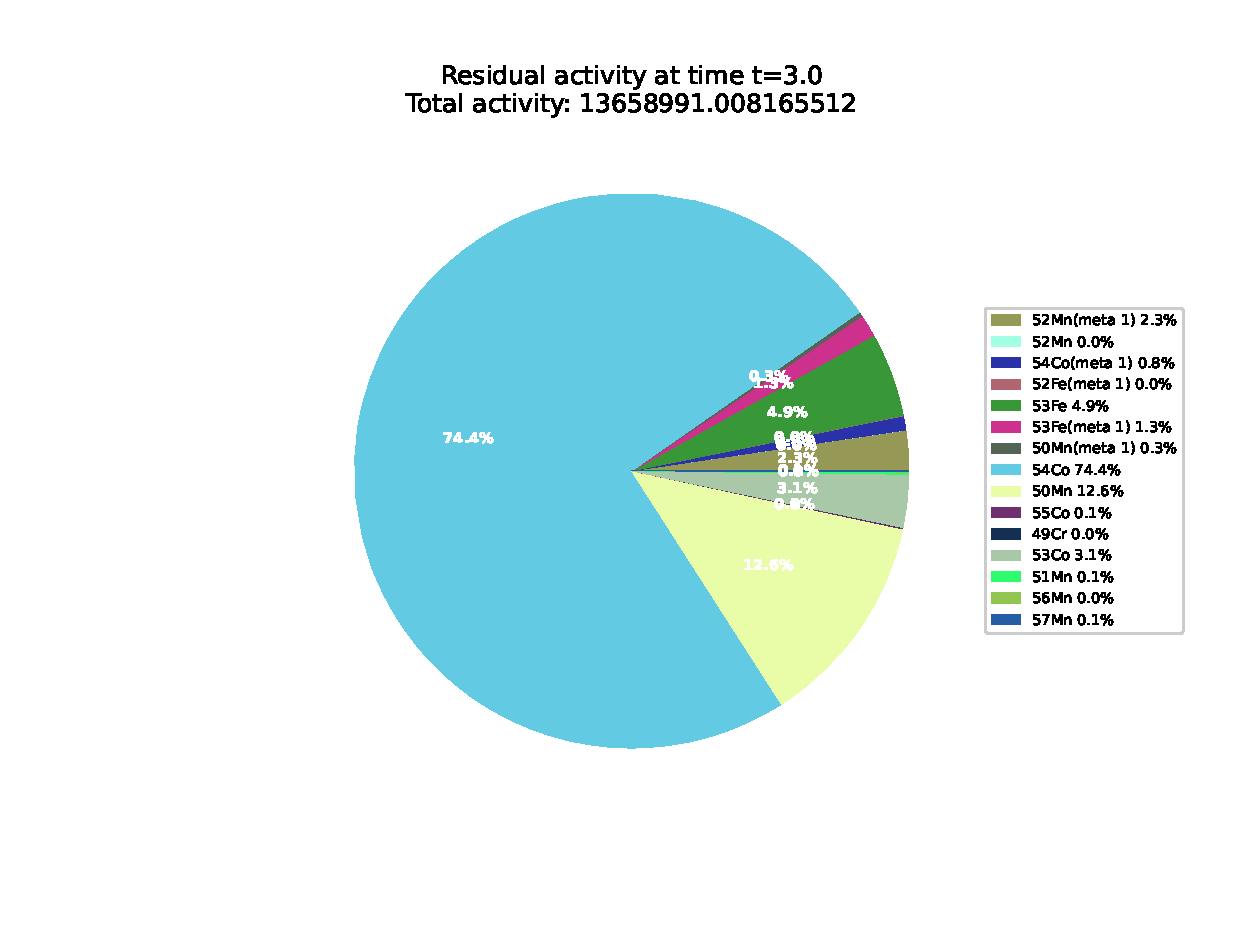
\includegraphics[width=0.8\linewidth]{chapters/activity_code/fe-activity-v2/residual-activity/0001_3.eps}
\caption{}
\label{fig:activity-v2-residual-activity-3s}
\end{figure}

\begin{figure}[!htb]
\centering
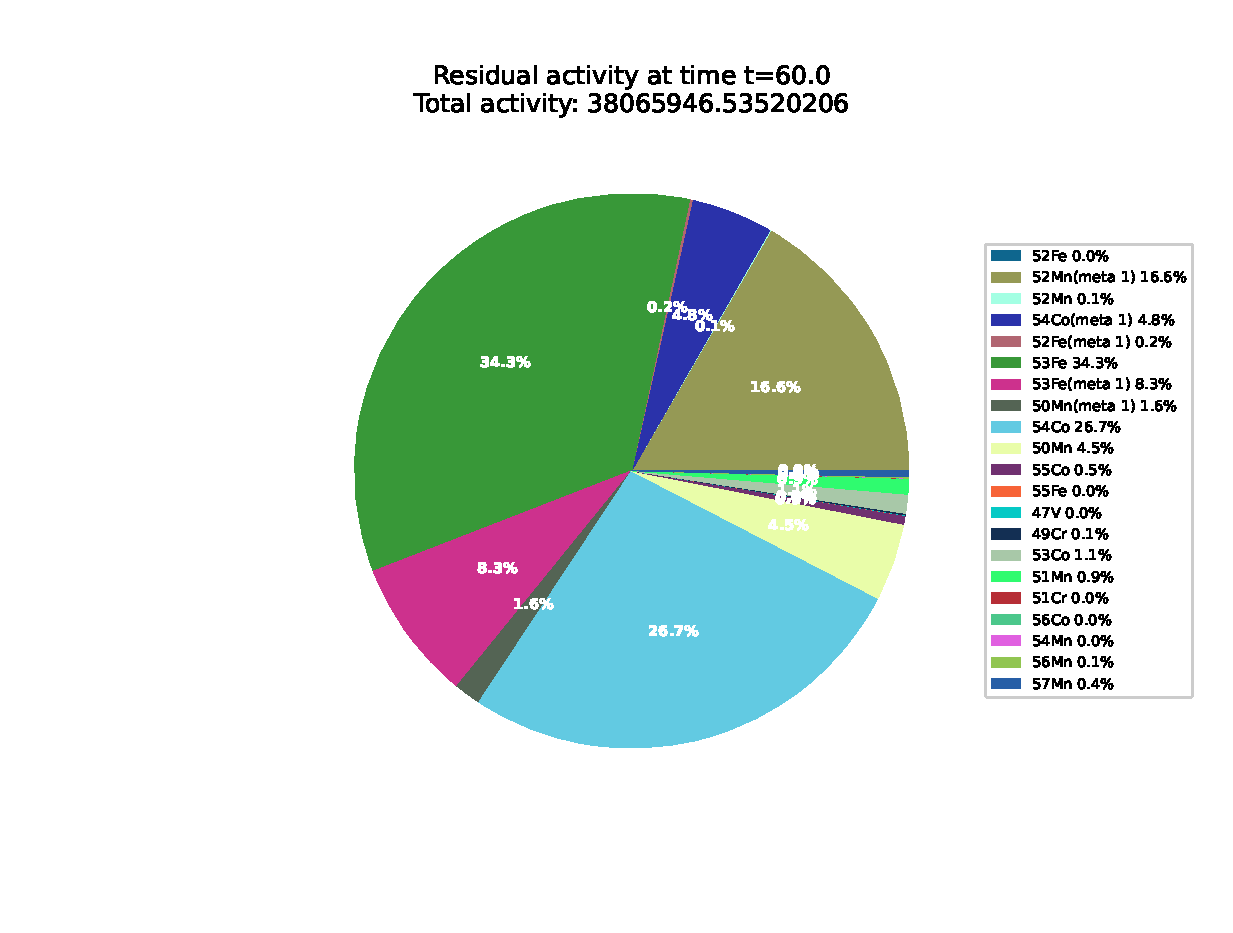
\includegraphics[width=0.8\linewidth]{chapters/activity_code/fe-activity-v2/residual-activity/0020_60.eps}
\caption{}
\label{fig:activity-v2-residual-activity-60s}
\end{figure}

\begin{figure}[!htb]
\centering
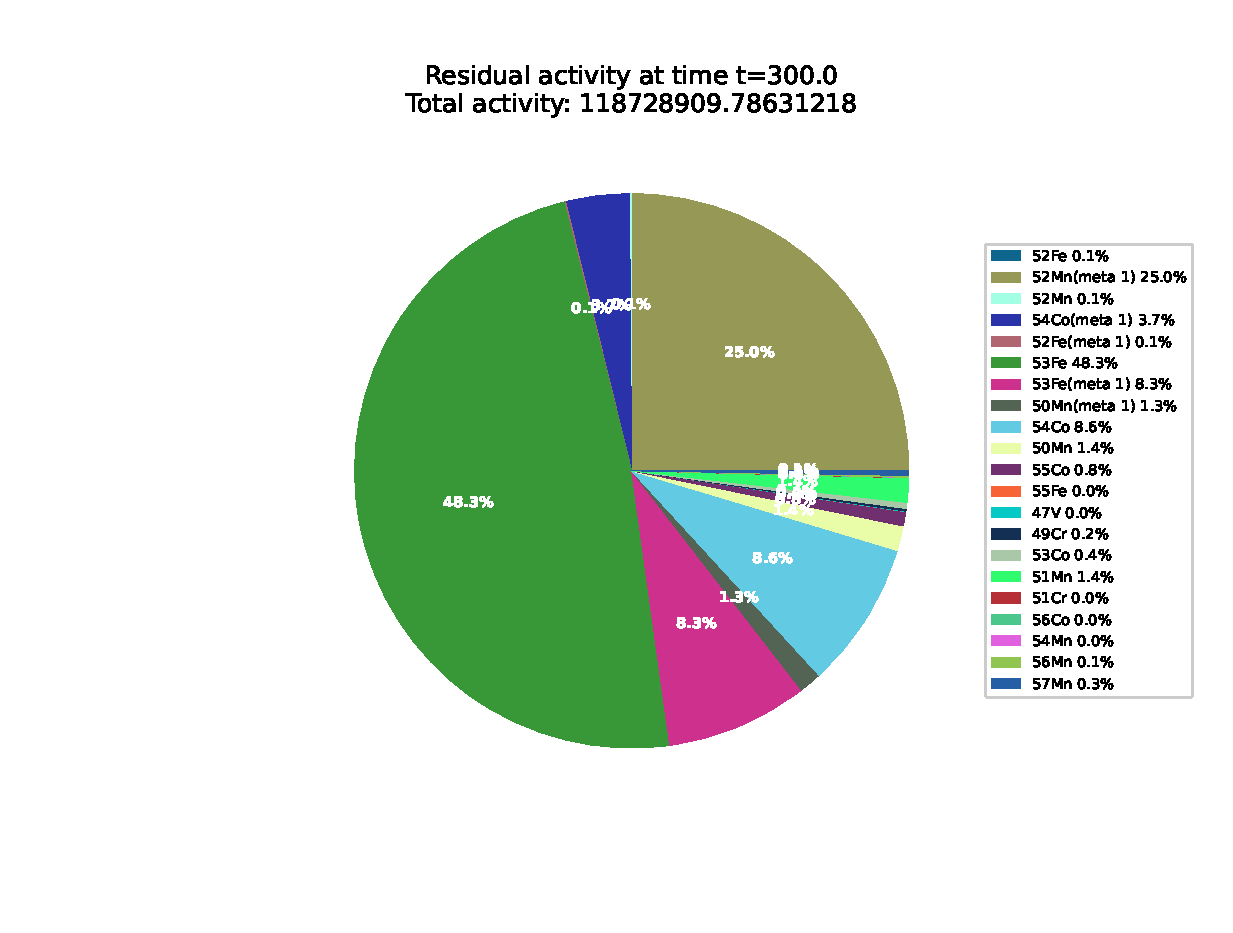
\includegraphics[width=0.8\linewidth]{chapters/activity_code/fe-activity-v2/residual-activity/0100_300.eps}
\caption{}
\label{fig:activity-v2-residual-activity-300s}
\end{figure}

\begin{figure}[!htb]
\centering
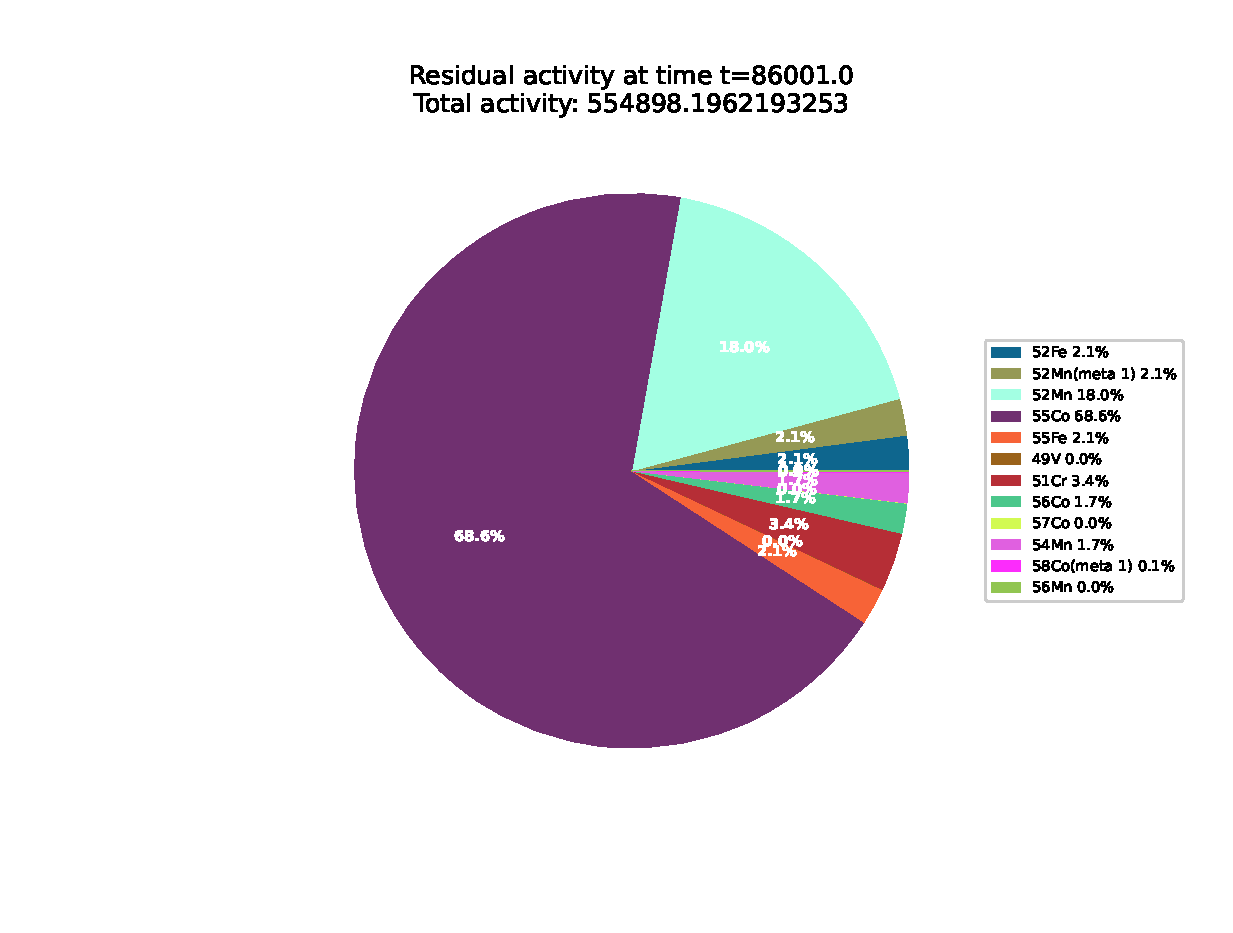
\includegraphics[width=0.8\linewidth]{chapters/activity_code/fe-activity-v2/residual-activity/0166_86001.eps}
\caption{}
\label{fig:activity-v2-residual-activity-86001s}
\end{figure}


\begin{figure}[!htb]
\centering
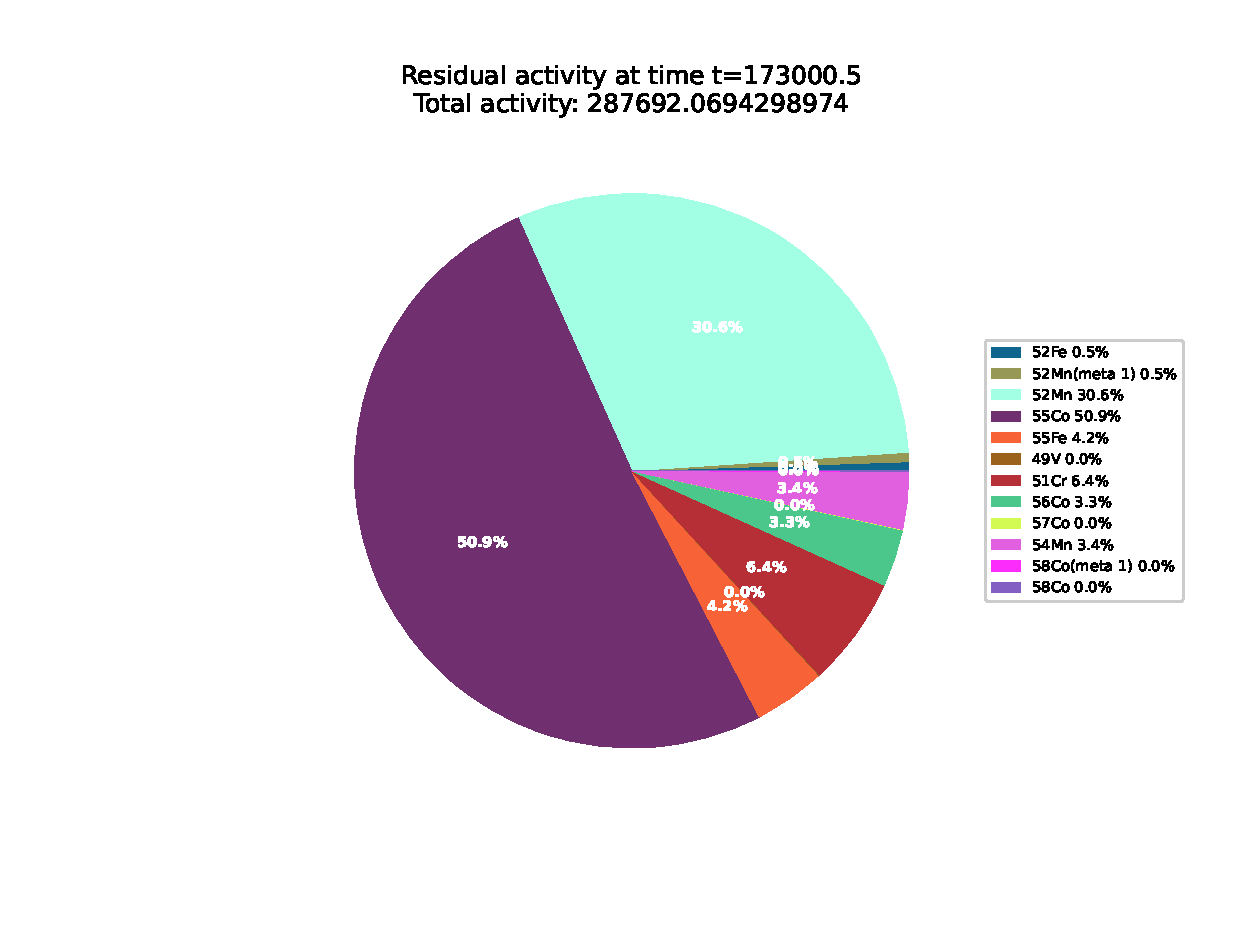
\includegraphics[width=0.8\linewidth]{chapters/activity_code/fe-activity-v2/residual-activity/0233_173000.eps}
\caption{}
\label{fig:activity-v2-residual-activity-173000s}
\end{figure}

\begin{figure}[!htb]
\centering
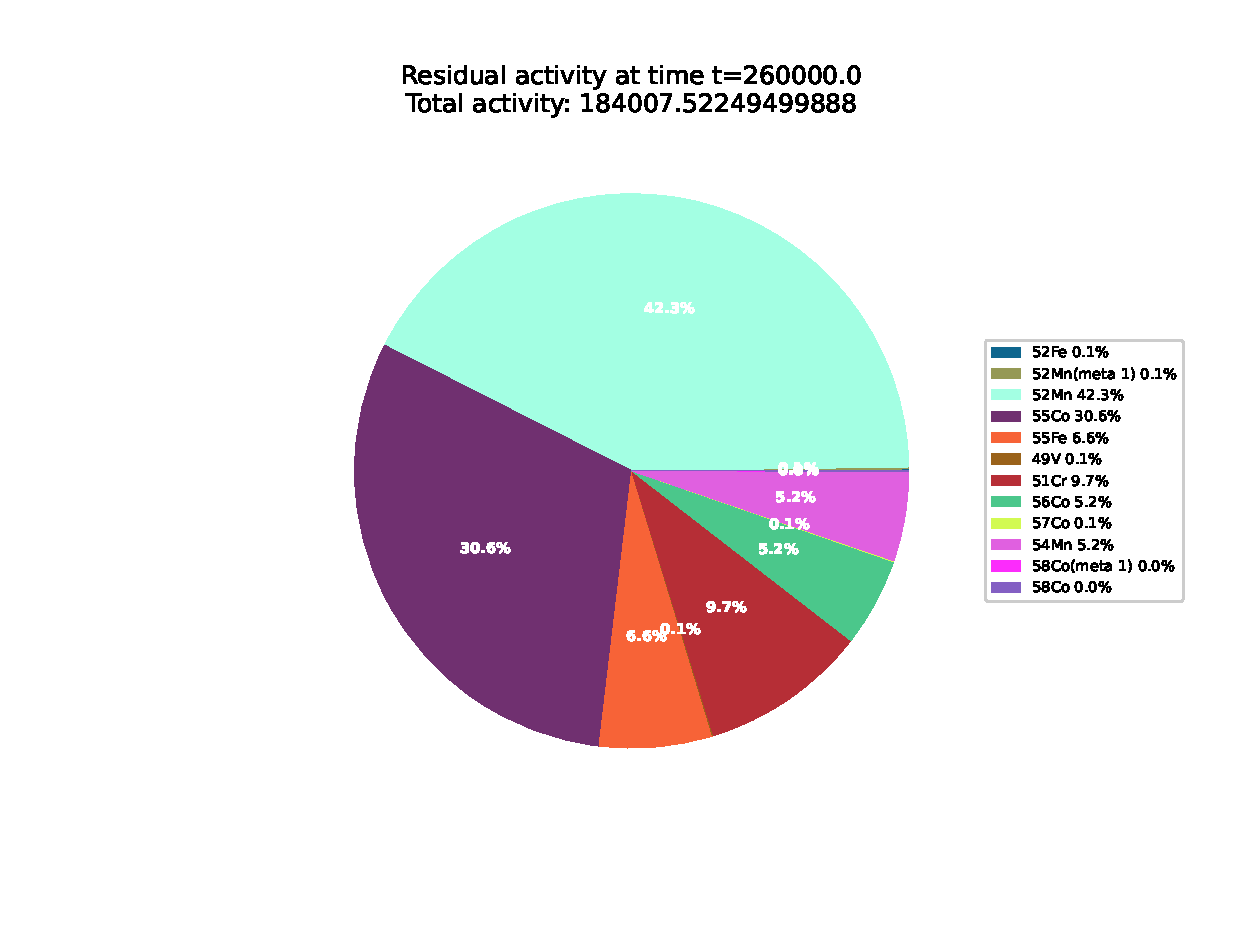
\includegraphics[width=0.8\linewidth]{chapters/activity_code/fe-activity-v2/residual-activity/0300_260000.eps}
\caption{}
\label{fig:activity-v2-residual-activity-260000s}
\end{figure}



\clearpage

\subsection{Gamma Output Tallied by Residual Isotope}

\FloatBarrier


\begin{figure}[!htb]
\centering
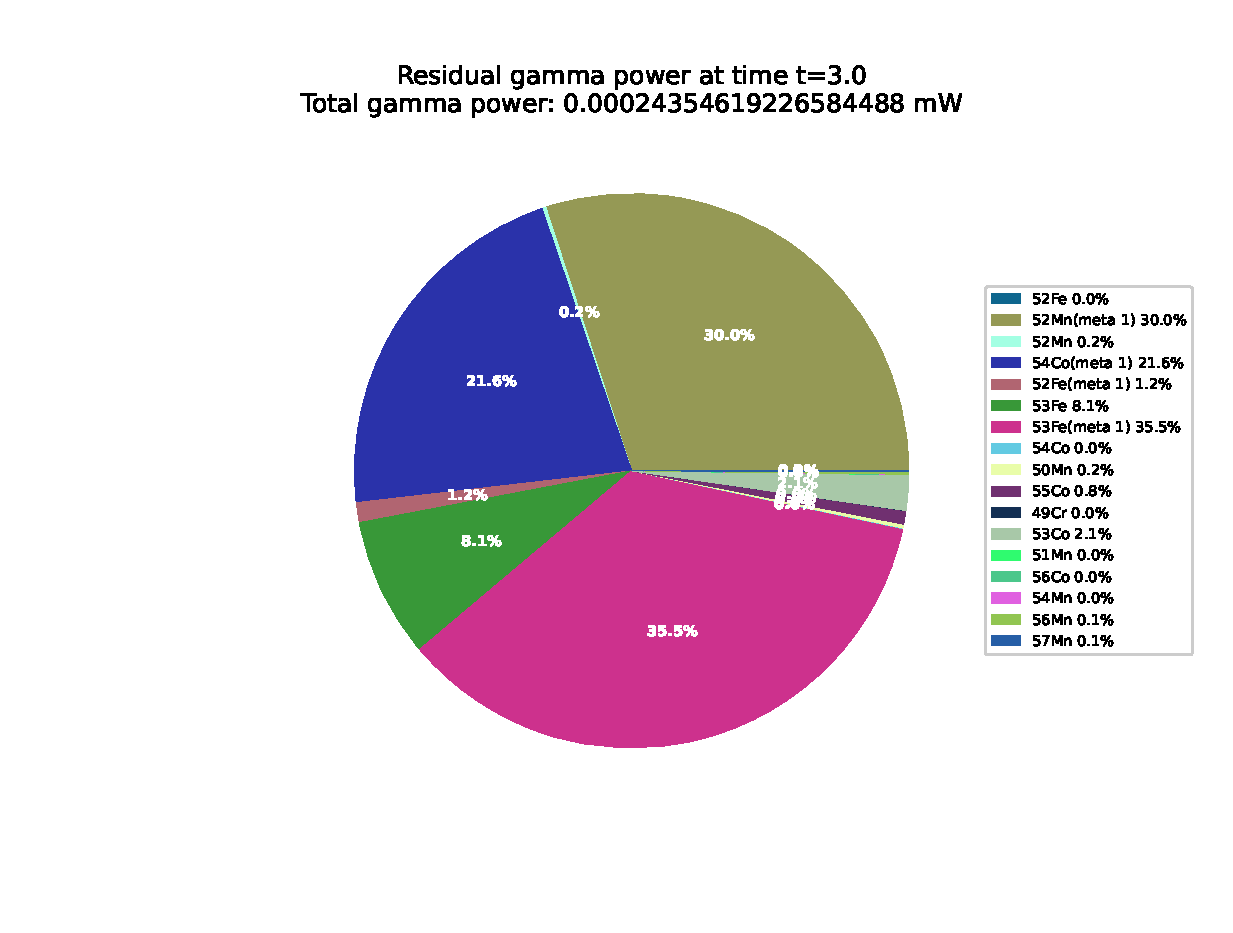
\includegraphics[width=0.8\linewidth]{chapters/activity_code/fe-activity-v2/residual-energy/0001_3.eps}
\caption{}
\label{fig:activity-v2-residual-power-3s}
\end{figure}

\begin{figure}[!htb]
\centering
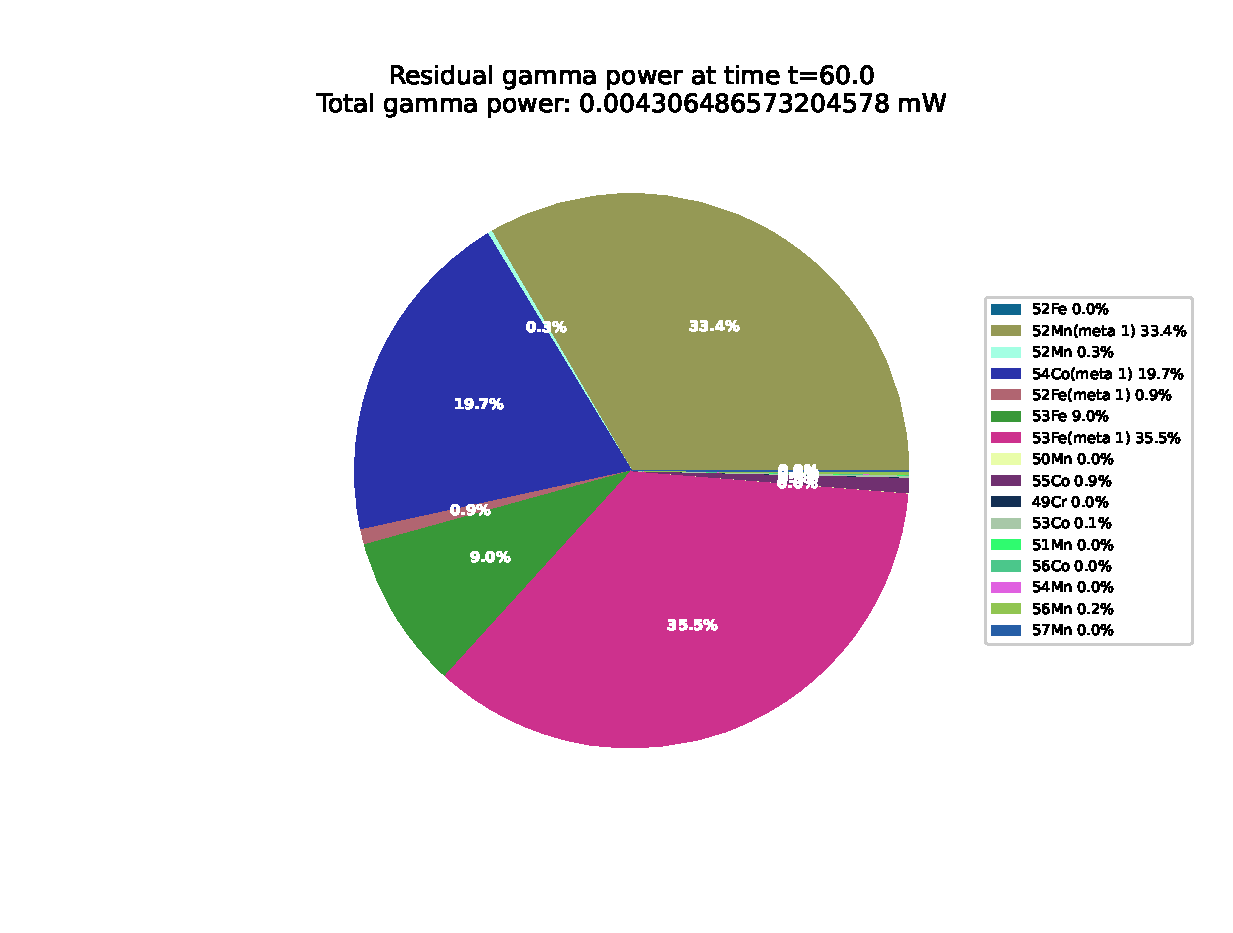
\includegraphics[width=0.8\linewidth]{chapters/activity_code/fe-activity-v2/residual-energy/0020_60.eps}
\caption{}
\label{fig:activity-v2-residual-power-60s}
\end{figure}

\begin{figure}[!htb]
\centering
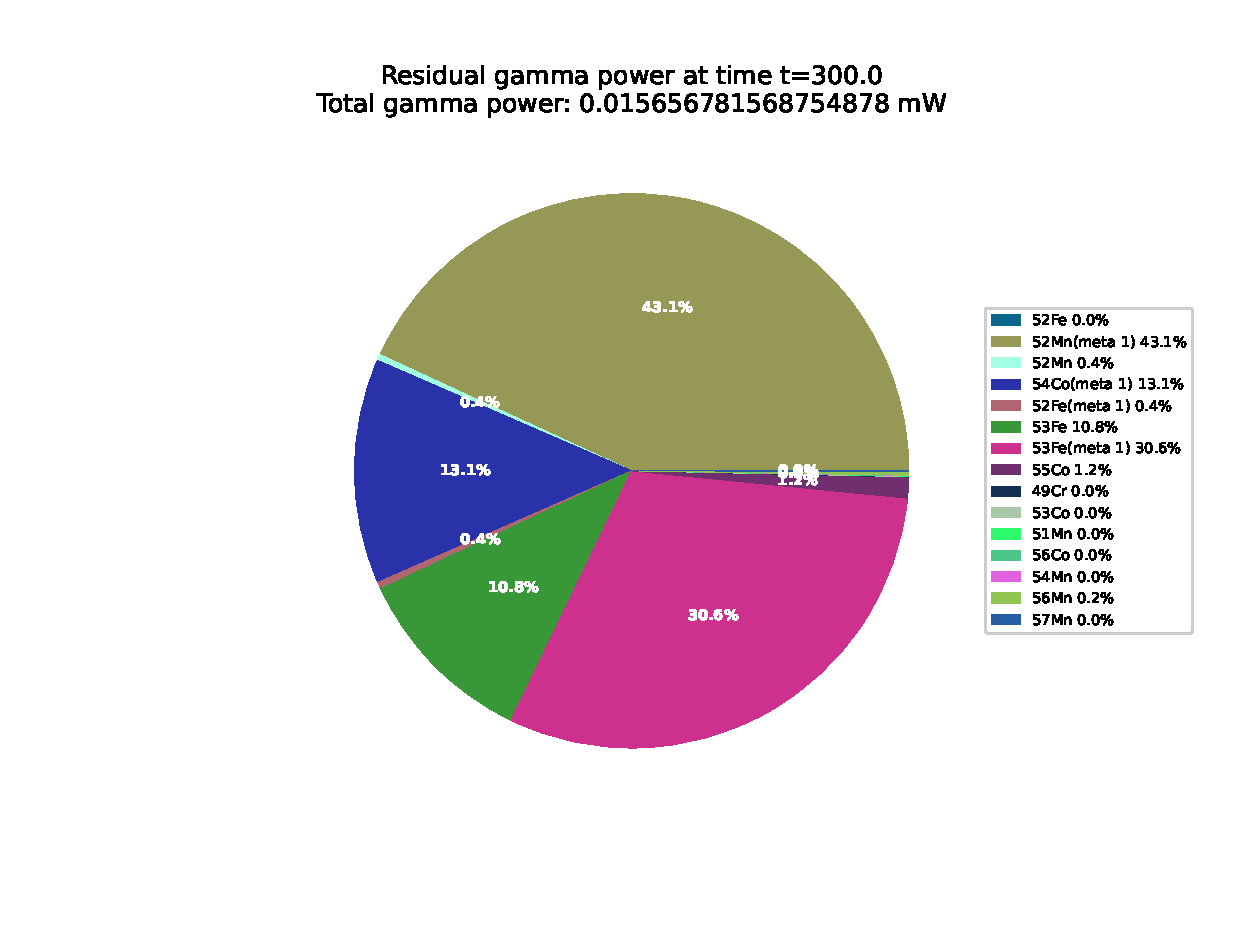
\includegraphics[width=0.8\linewidth]{chapters/activity_code/fe-activity-v2/residual-energy/0100_300.eps}
\caption{}
\label{fig:activity-v2-residual-power-300s}
\end{figure}

\begin{figure}[!htb]
\centering
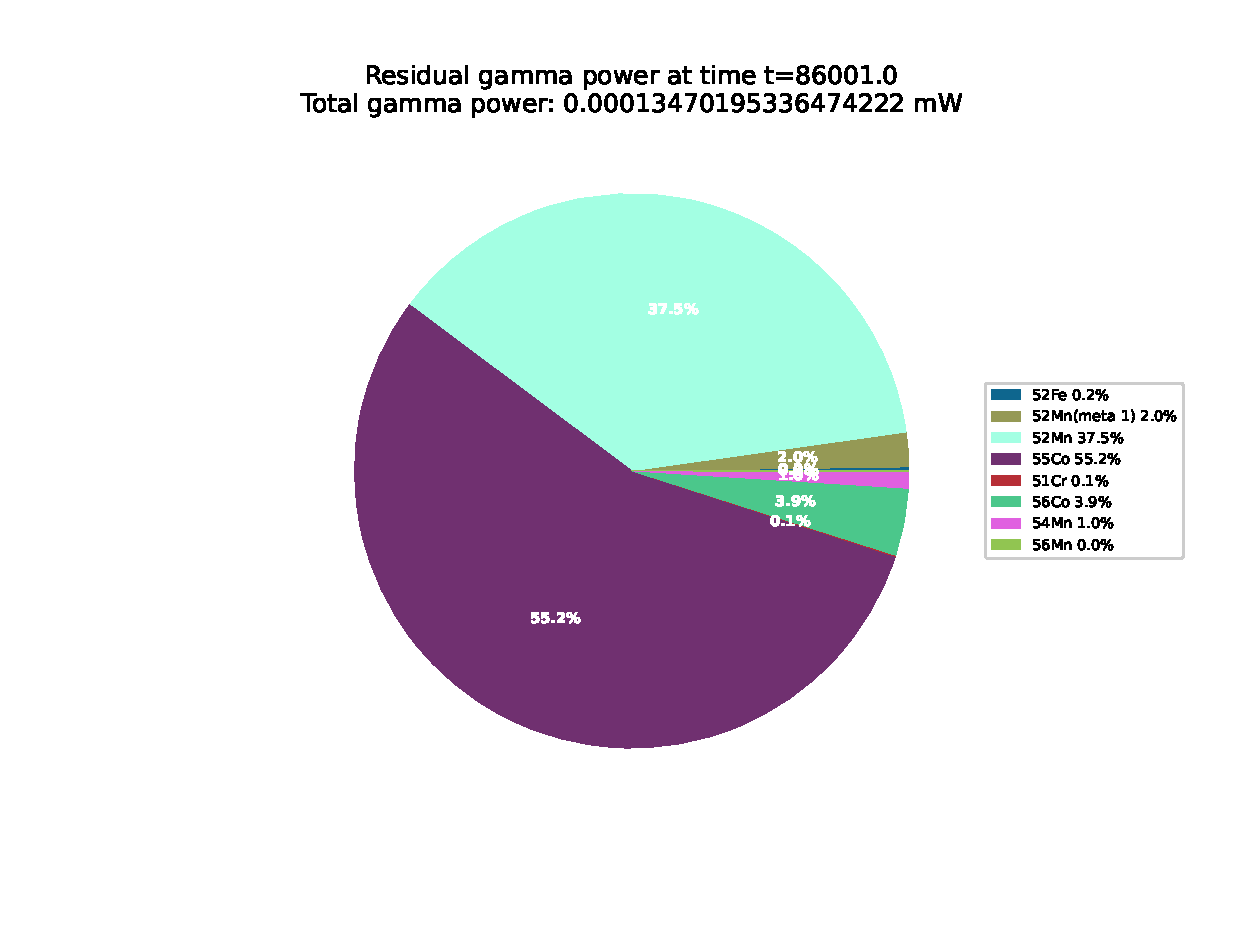
\includegraphics[width=0.8\linewidth]{chapters/activity_code/fe-activity-v2/residual-energy/0166_86001.eps}
\caption{}
\label{fig:activity-v2-residual-power-86001s}
\end{figure}

\begin{figure}[!htb]
\centering
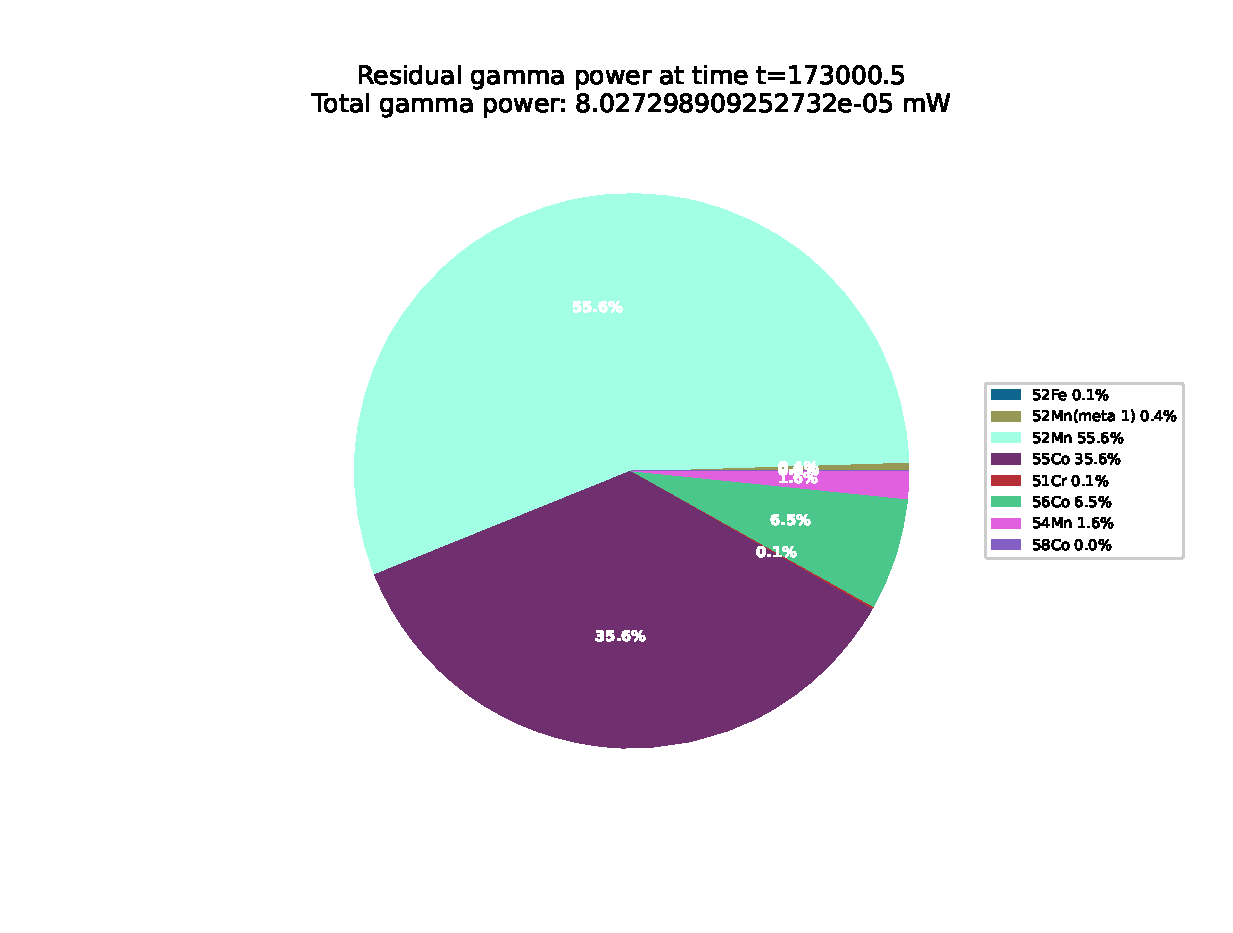
\includegraphics[width=0.8\linewidth]{chapters/activity_code/fe-activity-v2/residual-energy/0233_173000.eps}
\caption{}
\label{fig:activity-v2-residual-power-173000s}
\end{figure}

\begin{figure}[!htb]
\centering
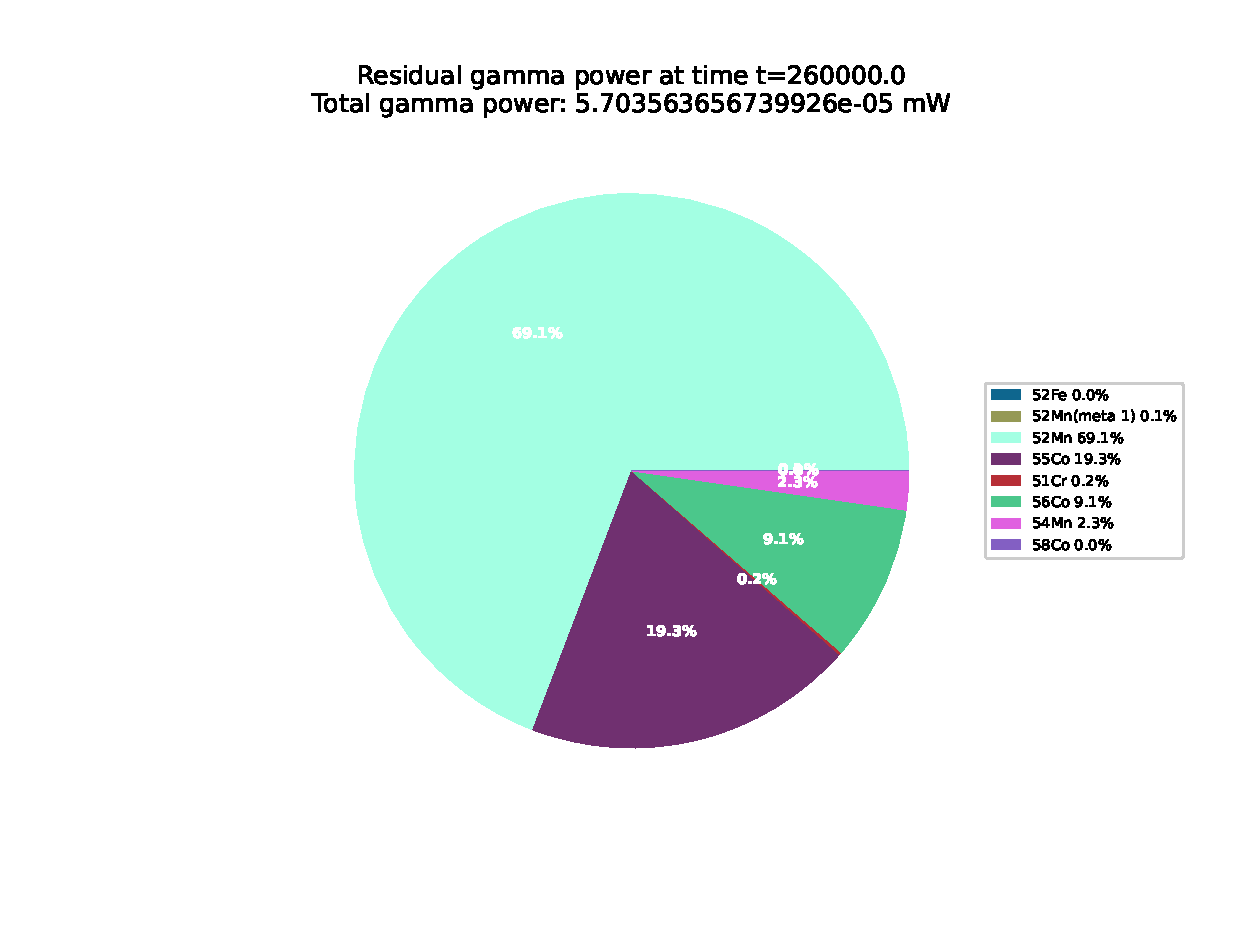
\includegraphics[width=0.8\linewidth]{chapters/activity_code/fe-activity-v2/residual-energy/0300_260000.eps}
\caption{}
\label{fig:activity-v2-residual-power-260000s}
\end{figure}



\clearpage

\subsection{Activity Tallied by Target Isotope}

\FloatBarrier


\begin{figure}[!htb]
\centering
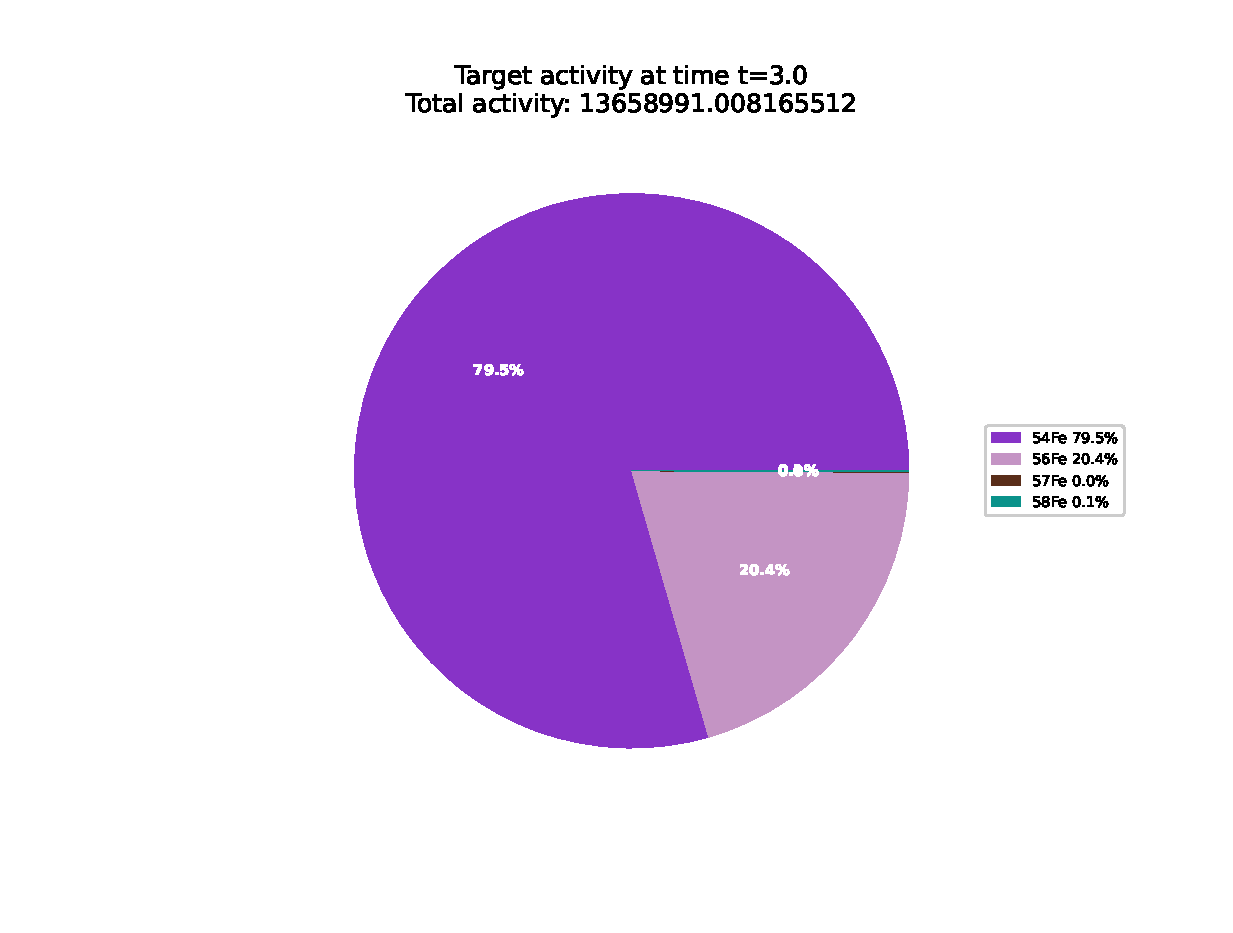
\includegraphics[width=0.8\linewidth]{chapters/activity_code/fe-activity-v2/target-activity/0001_3.eps}
\caption{}
\label{fig:activity-v2-target-activity-3s}
\end{figure}

\begin{figure}[!htb]
\centering
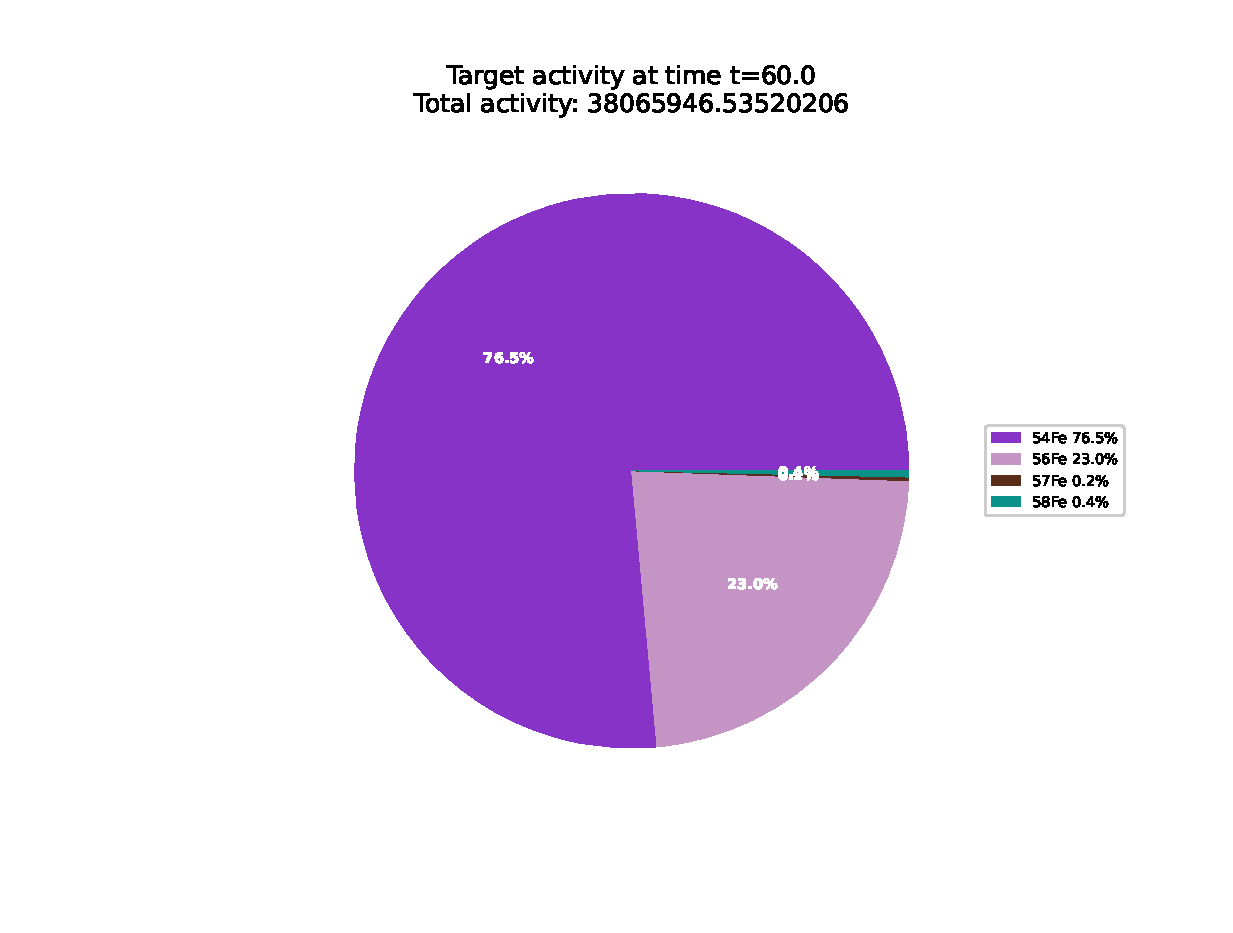
\includegraphics[width=0.8\linewidth]{chapters/activity_code/fe-activity-v2/target-activity/0020_60.eps}
\caption{}
\label{fig:activity-v2-target-activity-60s}
\end{figure}

\begin{figure}[!htb]
\centering
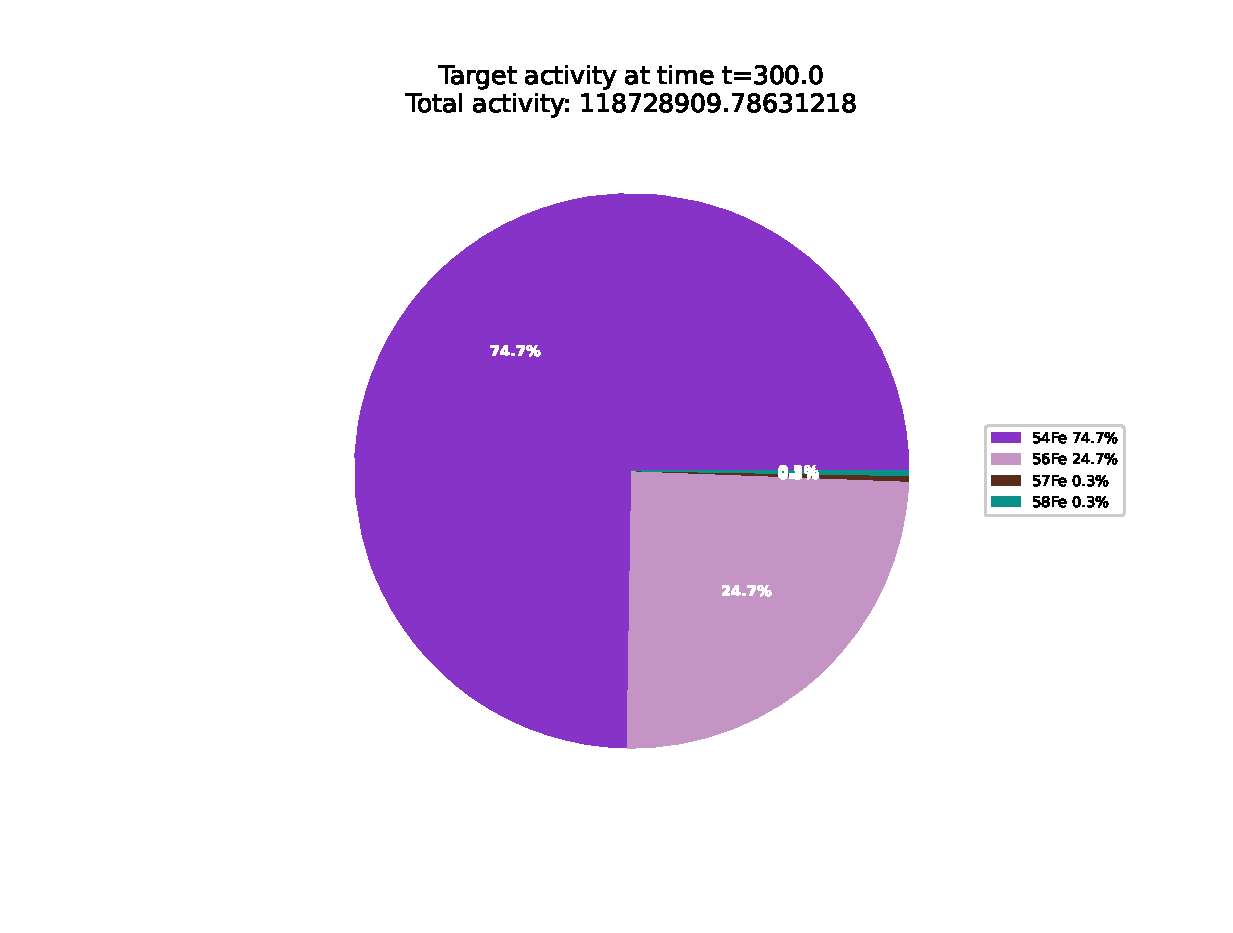
\includegraphics[width=0.8\linewidth]{chapters/activity_code/fe-activity-v2/target-activity/0100_300.eps}
\caption{}
\label{fig:activity-v2-target-activity-300s}
\end{figure}

\begin{figure}[!htb]
\centering
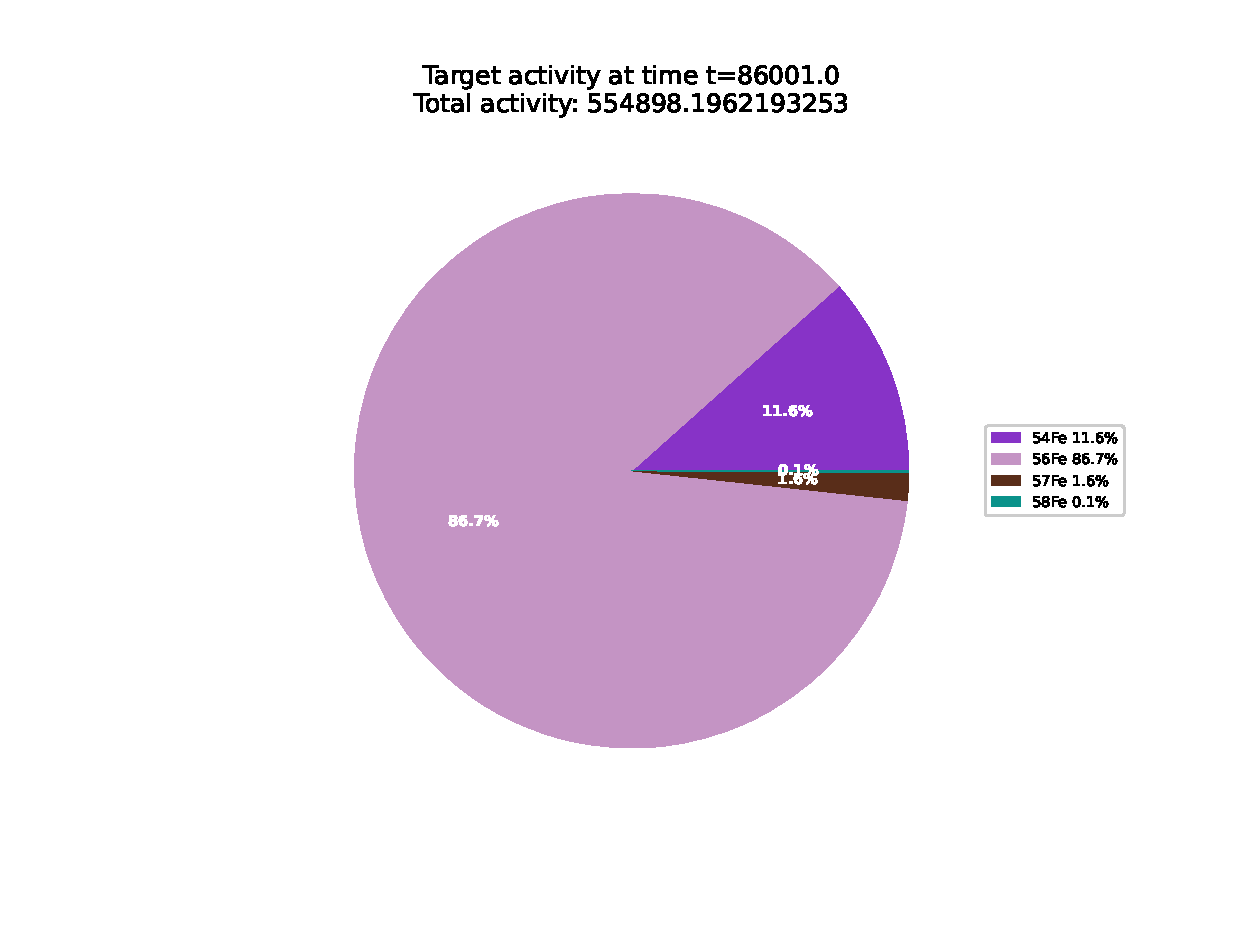
\includegraphics[width=0.8\linewidth]{chapters/activity_code/fe-activity-v2/target-activity/0166_86001.eps}
\caption{}
\label{fig:activity-v2-target-activity-86001s}
\end{figure}


\begin{figure}[!htb]
\centering
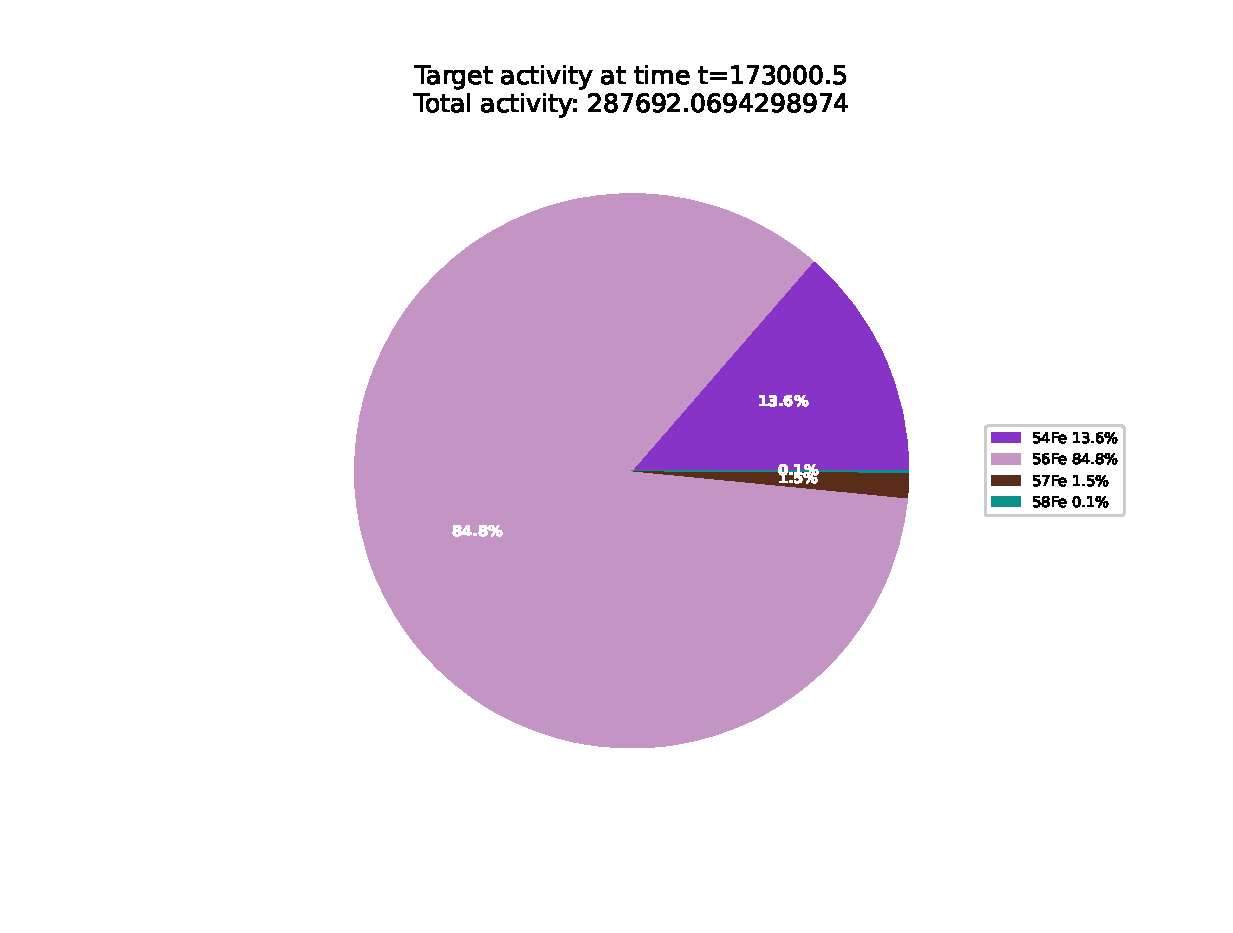
\includegraphics[width=0.8\linewidth]{chapters/activity_code/fe-activity-v2/target-activity/0233_173000.eps}
\caption{}
\label{fig:activity-v2-target-activity-173000s}
\end{figure}

\begin{figure}[!htb]
\centering
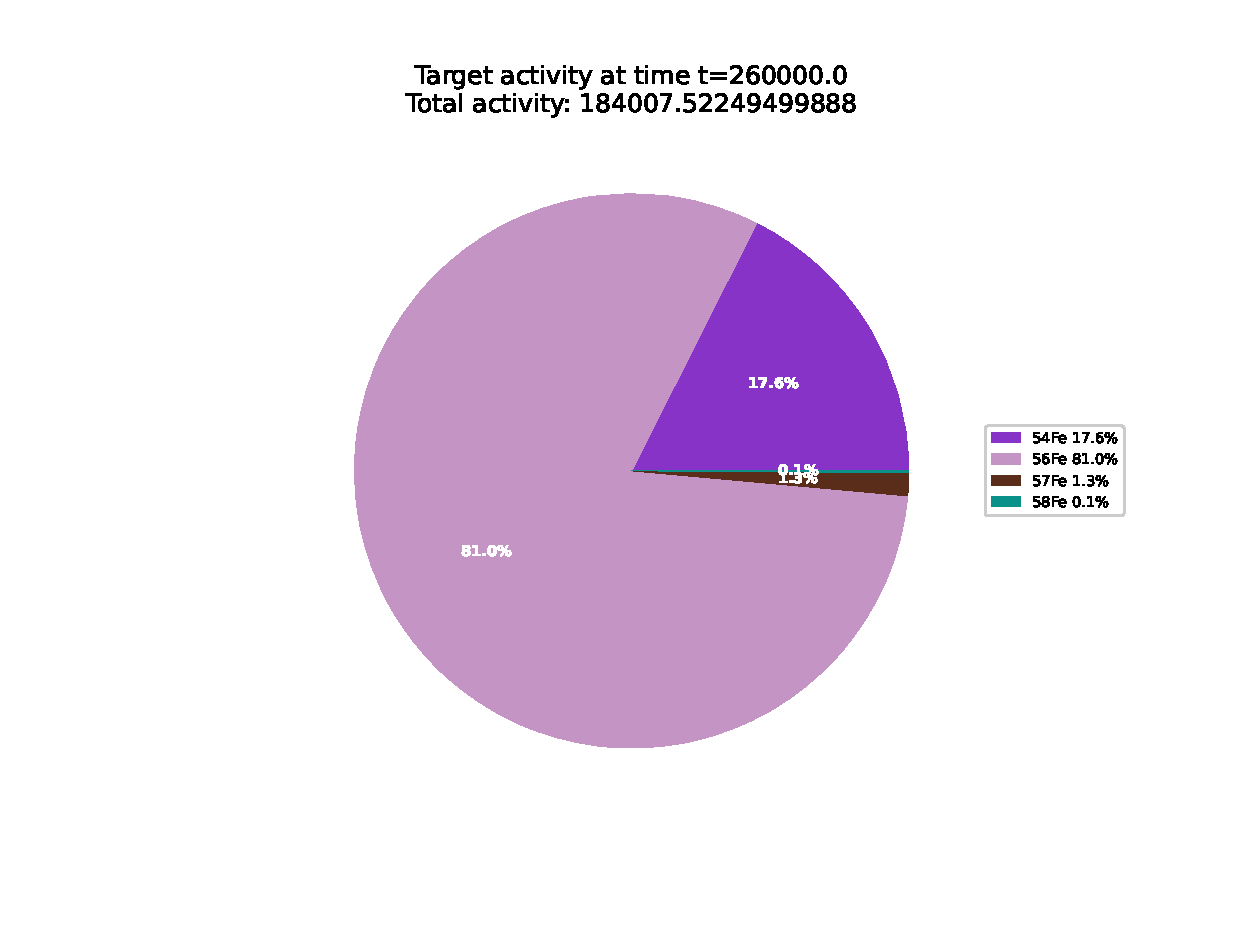
\includegraphics[width=0.8\linewidth]{chapters/activity_code/fe-activity-v2/target-activity/0300_260000.eps}
\caption{}
\label{fig:activity-v2-target-activity-260000s}
\end{figure}




\clearpage

\subsection{Gamma Output Tallied by Target Isotope}

\FloatBarrier


\begin{figure}[!htb]
\centering
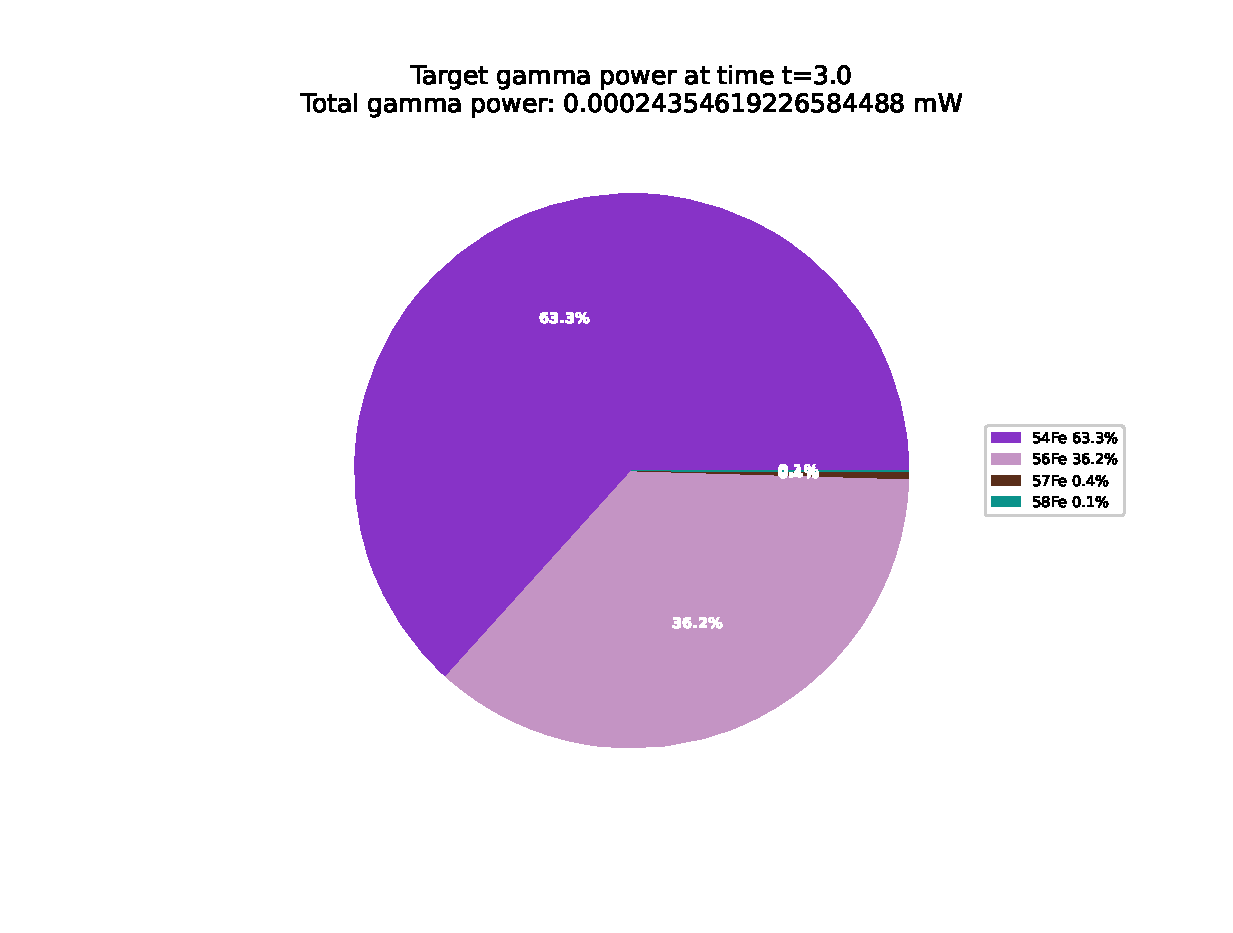
\includegraphics[width=0.8\linewidth]{chapters/activity_code/fe-activity-v2/target-energy/0001_3.eps}
\caption{}
\label{fig:activity-v2-target-power-3s}
\end{figure}

\begin{figure}[!htb]
\centering
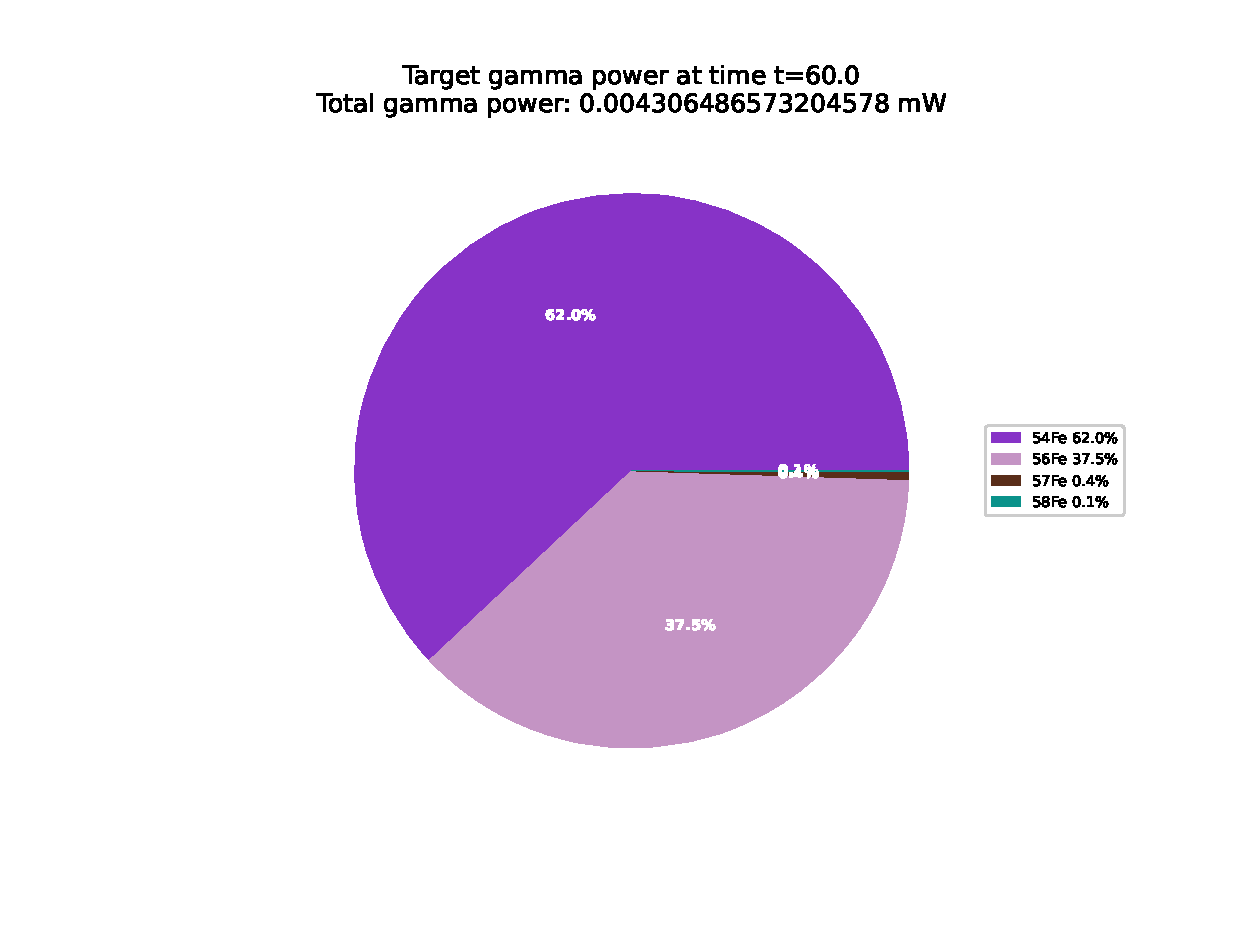
\includegraphics[width=0.8\linewidth]{chapters/activity_code/fe-activity-v2/target-energy/0020_60.eps}
\caption{}
\label{fig:activity-v2-target-power-60s}
\end{figure}

\begin{figure}[!htb]
\centering
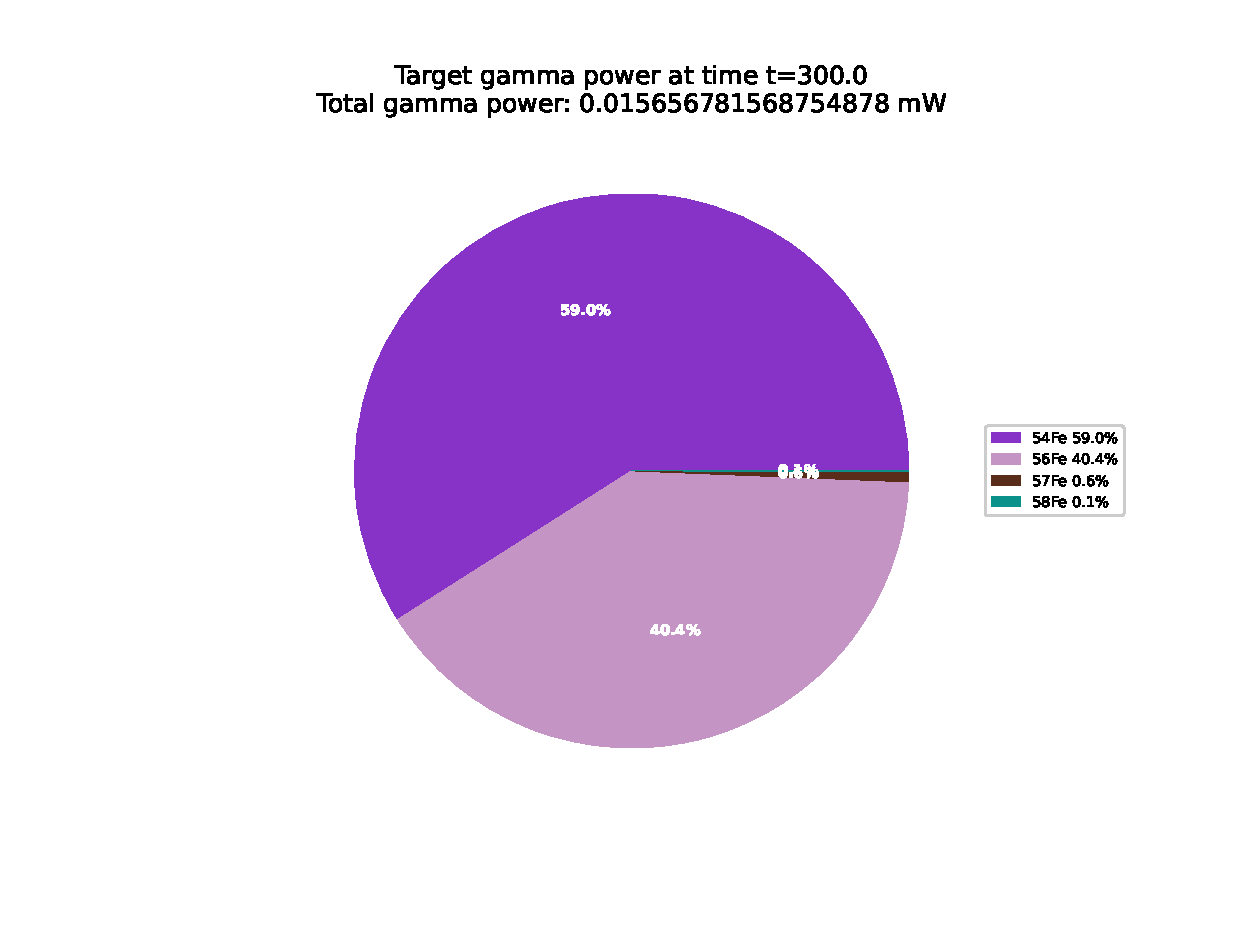
\includegraphics[width=0.8\linewidth]{chapters/activity_code/fe-activity-v2/target-energy/0100_300.eps}
\caption{}
\label{fig:activity-v2-target-power-300s}
\end{figure}

\begin{figure}[!htb]
\centering
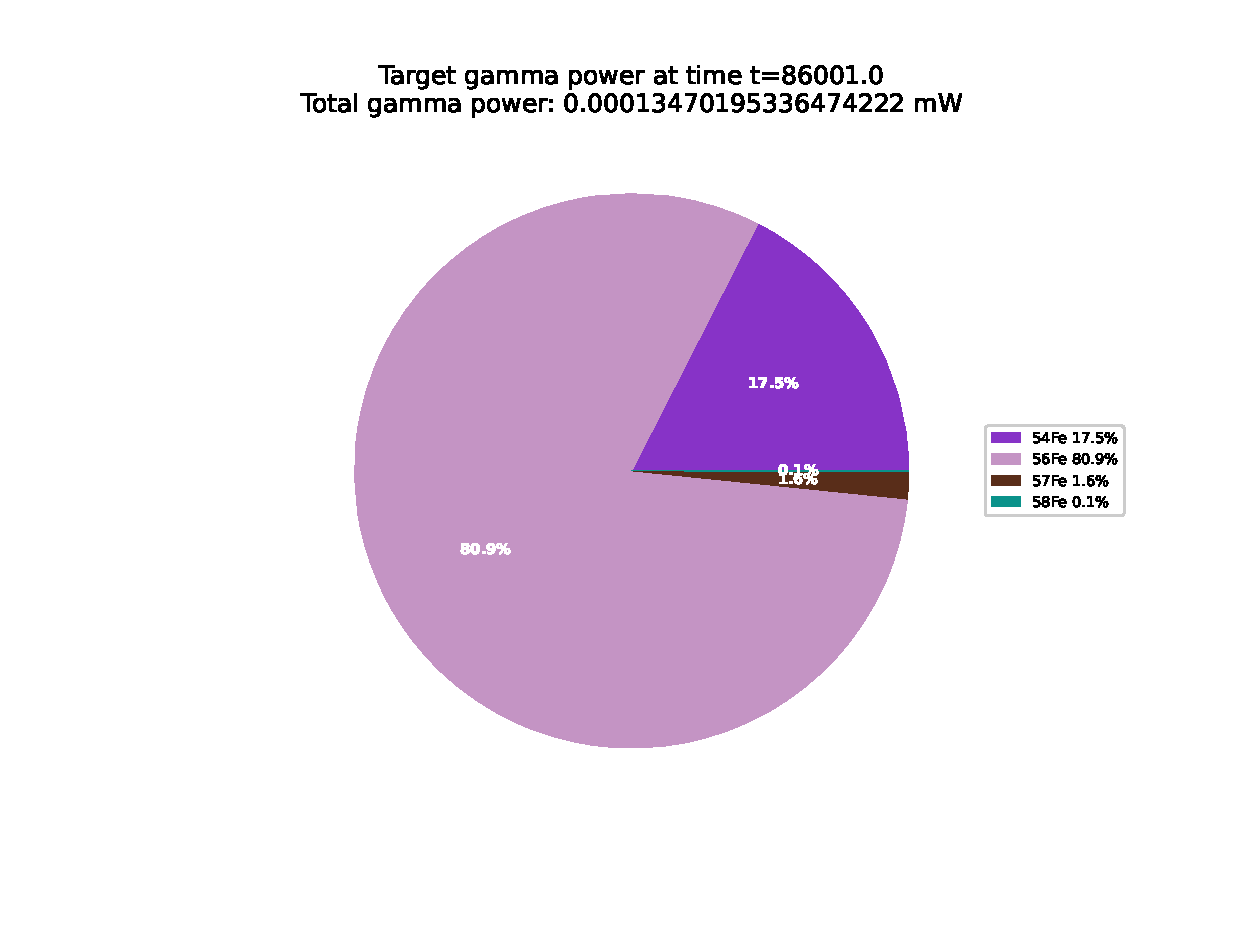
\includegraphics[width=0.8\linewidth]{chapters/activity_code/fe-activity-v2/target-energy/0166_86001.eps}
\caption{}
\label{fig:activity-v2-target-power-86001s}
\end{figure}

\begin{figure}[!htb]
\centering
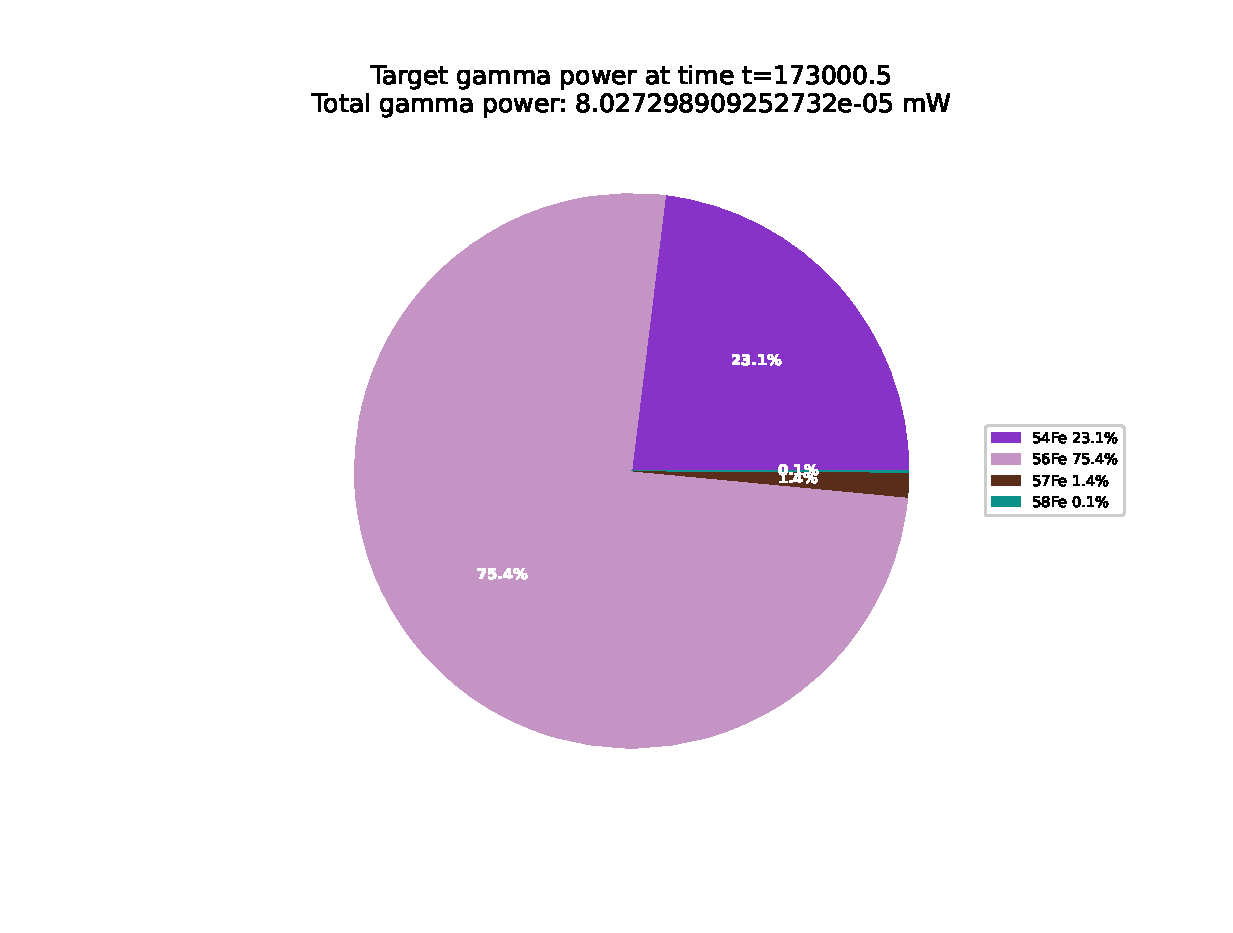
\includegraphics[width=0.8\linewidth]{chapters/activity_code/fe-activity-v2/target-energy/0233_173000.eps}
\caption{}
\label{fig:activity-v2-target-power-173000s}
\end{figure}

\begin{figure}[!htb]
\centering
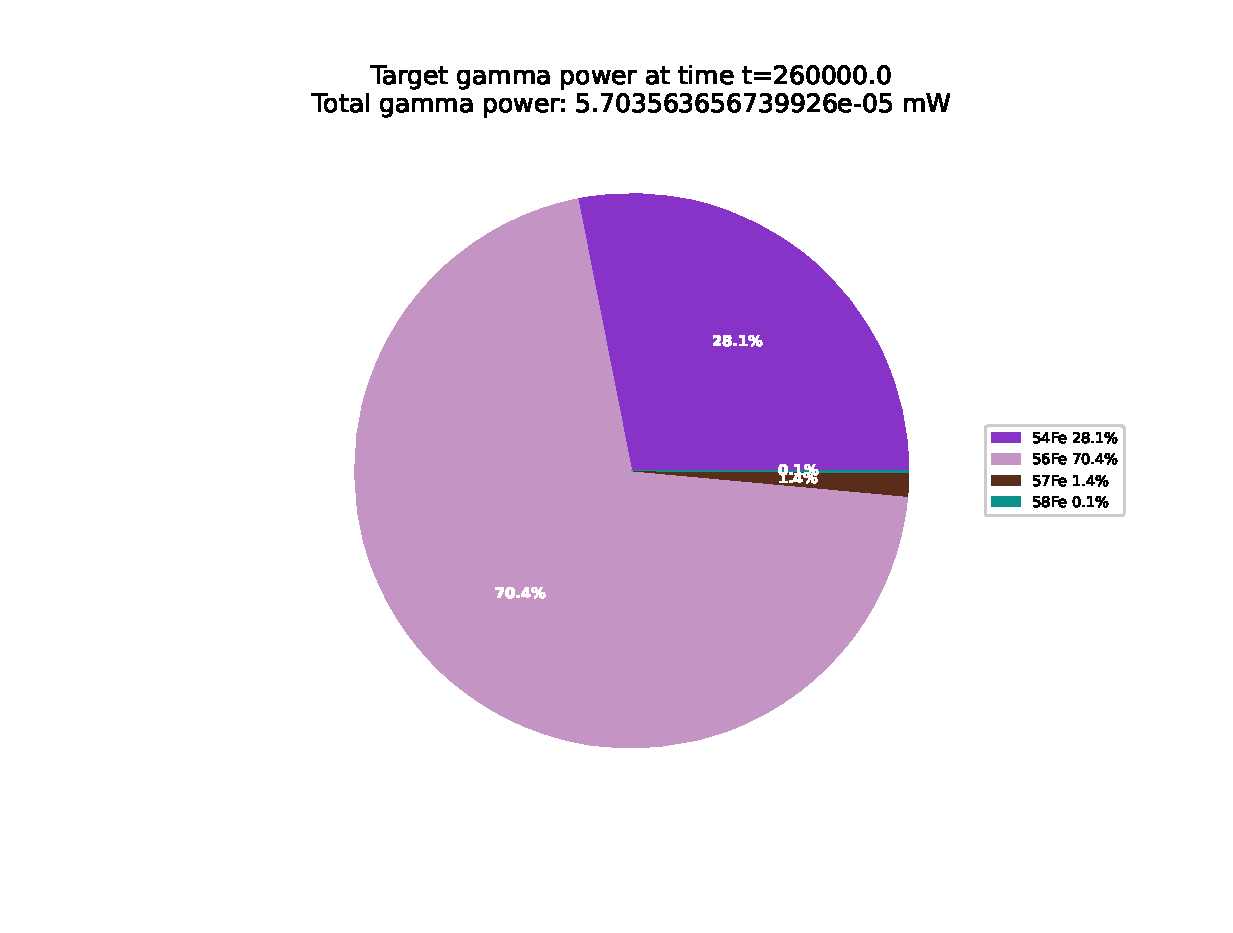
\includegraphics[width=0.8\linewidth]{chapters/activity_code/fe-activity-v2/target-energy/0300_260000.eps}
\caption{}
\label{fig:activity-v2-target-power-260000s}
\end{figure}


